\section{Archetype Analysis Findings}
\label{sec:archetype-findings}

This section reports the empirical findings of the archetype analysis whose
statistical design is described in \Cref{sec:archetype-analysis}. The
presentation follows the four-layer structure established there: descriptive
quartile profiles (\Cref{sec:descriptive-findings}), statistical confirmation
of the primary hypotheses (\Cref{sec:statistical-confirmation}), era-stratified
analysis (\Cref{sec:era-findings}), and quadrant analysis of elite team-seasons
(\Cref{sec:quadrant-findings}). The section closes with a hypothesis-testing
summary (\Cref{sec:hypothesis-summary}) that evaluates H1, H2, and H3 against
the evidence and assesses the overall claim that ``defense wins championships''
\parencite{robst2011defense}.

The unit of analysis throughout is the team-season. The full sample of
$n = 224$ team-seasons (32 teams, 7 seasons, 2018--2024) is used for
season-level analyses; the playoff subsample of $n = 94$ team-seasons is used
where outcomes are conditioned on postseason qualification. All independent
variables are defined in \Cref{tab:ivs} and all dependent variables in
\Cref{tab:dvs}.

% ============================================================
\subsection{Descriptive Findings}
\label{sec:descriptive-findings}
% ============================================================

\subsubsection{Offense Share Quartiles}
\label{sec:offense-share-quartiles}

The primary descriptive analysis partitions all 224 team-seasons into four
equal groups (56 per quartile) by \texttt{offense\_share}, as specified in
\Cref{sec:quartile-analysis}. Quartile~1 (Q1) contains the most
defense-dominant team-seasons (most negative \texttt{offense\_share}) and
Quartile~4 (Q4) contains the most offense-dominant. \Cref{tab:quartile-offense}
reports playoff appearance rates, mean playoff wins, conference championship
appearance rates, and Super Bowl win counts for each quartile.

\begin{table}[htbp]
  \centering
  \caption{Postseason outcomes by \texttt{offense\_share} quartile ($N = 224$
           team-seasons, 2018--2024; 56 per quartile). Avg~PW includes
           non-qualifiers (playoff wins $= 0$). Conf+ is conference
           championship or better.}
  \label{tab:quartile-offense}
  \begin{adjustbox}{max width=\textwidth}
  \begin{tabular}{lcrrrrrr}
    \toprule
    \textbf{Quartile} & \textbf{N}
      & \textbf{Avg Share} & \textbf{Playoff\%}
      & \textbf{Avg PW} & \textbf{Conf+\%} & \textbf{SB Win\%} \\
    \midrule
    Q1 (Defense) & 56 & $-0.373$ & 10.7           & 0.02 & \phantom{0}0.0 & 0.0 \\
    Q2           & 56 & $+0.291$ & 14.3           & 0.05 & \phantom{0}0.0 & 0.0 \\
    Q3           & 56 & $+0.569$ & 55.4           & 0.46 & 12.5           & 1.8 \\
    Q4 (Offense) & 56 & $+0.815$ & 87.5           & 1.02 & 28.6           & 10.7 \\
    \bottomrule
  \end{tabular}
  \end{adjustbox}
\end{table}

\Cref{fig:quartile-bars} visualizes this gradient.

\begin{figure}[htbp]
  \centering
  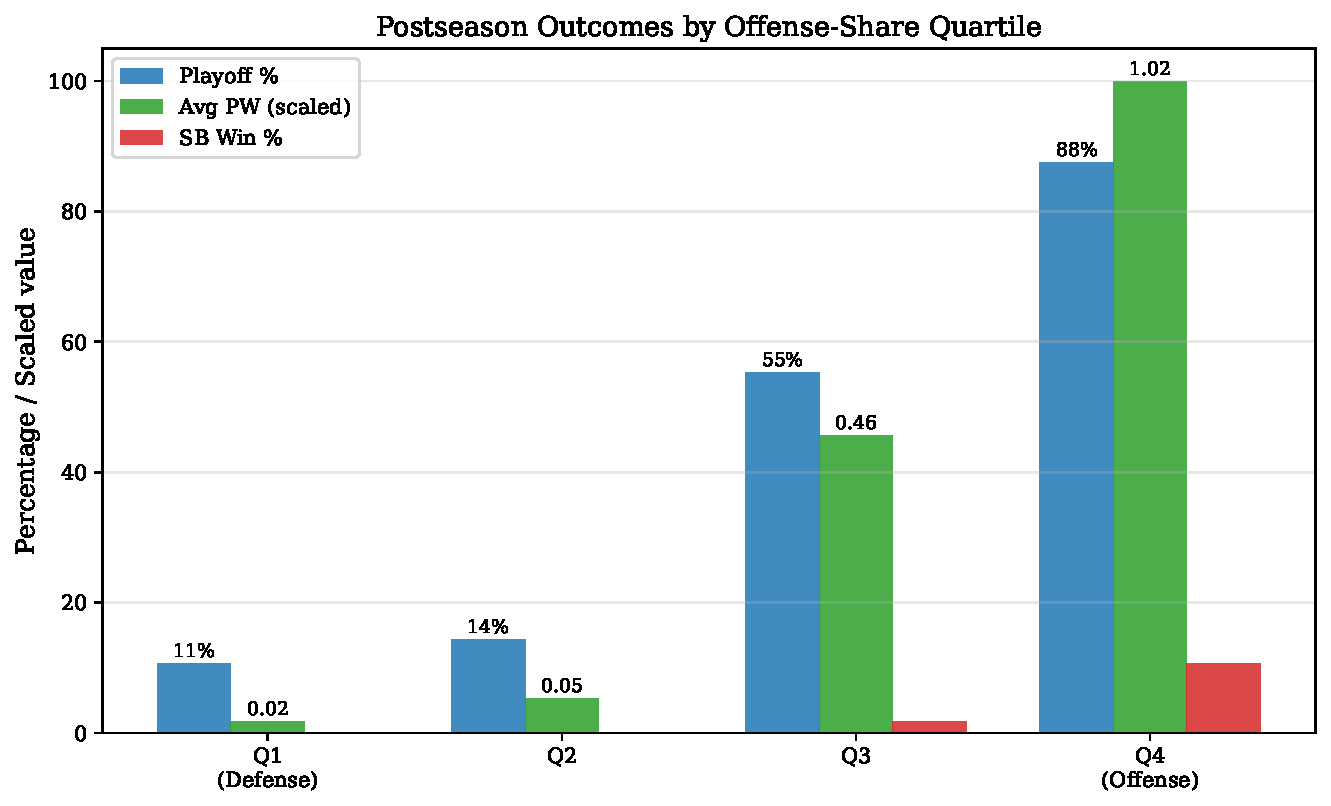
\includegraphics[width=0.85\textwidth]{figures/fig4_quartile_bars.pdf}
  \caption{Postseason outcomes by offense-share quartile. The monotonic
           gradient from Q1 (defense-dominant) to Q4 (offense-dominant) is
           visible across all three metrics: playoff qualification,
           average playoff wins, and Super Bowl victories.}
  \label{fig:quartile-bars}
\end{figure}

The data reveal a monotonic gradient that runs in precisely the opposite
direction to that predicted by the ``defense wins championships'' narrative.
Playoff appearance rates increase sharply and continuously from Q1 to Q4:
10.7\% of the most defense-dominant teams made the playoffs, compared to 87.5\%
of the most offense-dominant -- an eight-fold difference. Mean playoff wins follow
the same gradient, from 0.02 in Q1 to 1.02 in Q4. The gradient is not merely
linear but accelerating: the gap between Q3 and Q4 (0.46 to 1.02) is larger in
absolute terms than the gap between Q1 and Q2 (0.02 to 0.05), suggesting
convexity in the relationship between offensive dominance and playoff advancement.

The conference championship rate provides the starkest illustration of the
asymmetry. Not a single team-season in Q1 or Q2 -- collectively the 112 most
defense-dominant team-seasons in the dataset -- reached a conference
championship game. The first non-zero conference championship rate appears only
in Q3, at 12.5\%, and Q4 registers 28.6\%. Super Bowl victories are similarly
concentrated: all seven Super Bowl wins in the sample fall in Q3 or Q4; none
is attributable to a team in the two most defense-dominant quartiles.

No team-season in Q1 or Q2 reached a conference championship game or won a
Super Bowl. The complete absence of deep postseason runs in the two most
defense-dominant quartiles is notable given the large sample size ($n = 112$
team-seasons in Q1 and Q2 combined).

\subsubsection{Overall Team Quality Quartiles}
\label{sec:gds-quartiles}

A complementary quartile analysis partitions all 224 team-seasons by overall
\gds{}/game, producing tiers labeled Bottom, Below Average, Above Average, and
Top. \Cref{tab:quartile-gds} reports postseason outcomes for each tier.

\begin{table}[htbp]
  \centering
  \caption{Postseason outcomes by \gds{}/game quartile (overall team quality)
           across all 224 team-seasons (2018--2024). Each tier contains 56
           team-seasons. Avg PW is the unconditional mean of playoff wins
           across all team-seasons in the tier.}
  \label{tab:quartile-gds}
  \begin{tabular}{lcrrrr}
    \toprule
    \textbf{Tier} & \textbf{N}
      & \textbf{Playoff\%} & \textbf{Avg PW}
      & \textbf{Conf+\%} & \textbf{SB Win\%} \\
    \midrule
    Bottom     & 56 & \phantom{0}0.0 & 0.00 & 0.0 & 0.0 \\
    Below Avg  & 56 & 21.4           & 0.07 & 0.0 & 0.0 \\
    Above Avg  & 56 & 50.0           & 0.27 & 5.4 & 0.0 \\
    Top        & 56 & 96.4           & 1.21 & 35.7 & 12.5 \\
    \bottomrule
  \end{tabular}
\end{table}

The \gds{} strength gradient is even steeper than the offense-share gradient.
Teams in the top tier qualified for the playoffs in 96.4\% of team-seasons and
averaged 1.21 playoff wins, while no bottom-tier team made the playoffs at all.
The practical implication is that overall team quality -- the
total \gds{} signal -- is a powerful discriminant of postseason success at
every level of the outcome hierarchy: no bottom or below-average team reached
a conference championship game across 112 combined team-seasons.

Comparing \Cref{tab:quartile-gds} with \Cref{tab:quartile-offense} is
instructive. The \gds{} strength gradient is steeper than the offense-share
gradient at the bottom (Bottom at 0.0\% vs Q1 at 10.7\% for playoff rates;
Top at 96.4\% vs Q4 at 87.5\%), confirming that \emph{how good} a team is
matters more than \emph{whether the team is offense or defense oriented}.
However, among teams of similarly elevated overall quality, the subsequent
quadrant analysis (\Cref{sec:quadrant-findings}) reveals that the
offense-versus-defense balance within that quality level still carries
meaningful information about championship potential.

\subsubsection{Defense-Dominant Teams and Deep Playoff Runs}
\label{sec:myth-check}

A direct operationalization of the ``defense wins championships'' claim is the
prevalence of defense-dominant teams among playoff participants. Among the 94
playoff team-seasons in the dataset, only six have negative
\texttt{offense\_share} values (indicating net defense-dominant profiles),
and only one -- Pittsburgh 2023 ($\texttt{offense\_share} = -0.631$) -- has a
substantially defense-dominant profile ($\texttt{offense\_share} < -0.3$).
That team was eliminated in the first round (zero playoff wins).
This finding is stated plainly as the empirical headline of the analysis:
\textbf{no defense-dominant team (offense share $< 0$) won more than one
playoff game across seven seasons and 94 playoff team-seasons}. The sole
team to win any was Houston 2024 ($\texttt{offense\_share} = -0.069$, one
playoff win).
The near-total absence of defense-dominant teams from the playoff field -- and
their complete absence from deep postseason runs -- represents a more sweeping
finding than initially hypothesized. \Cref{fig:offense-share-pw} displays
this relationship visually, with Super Bowl winners annotated.

\begin{figure}[htbp]
  \centering
  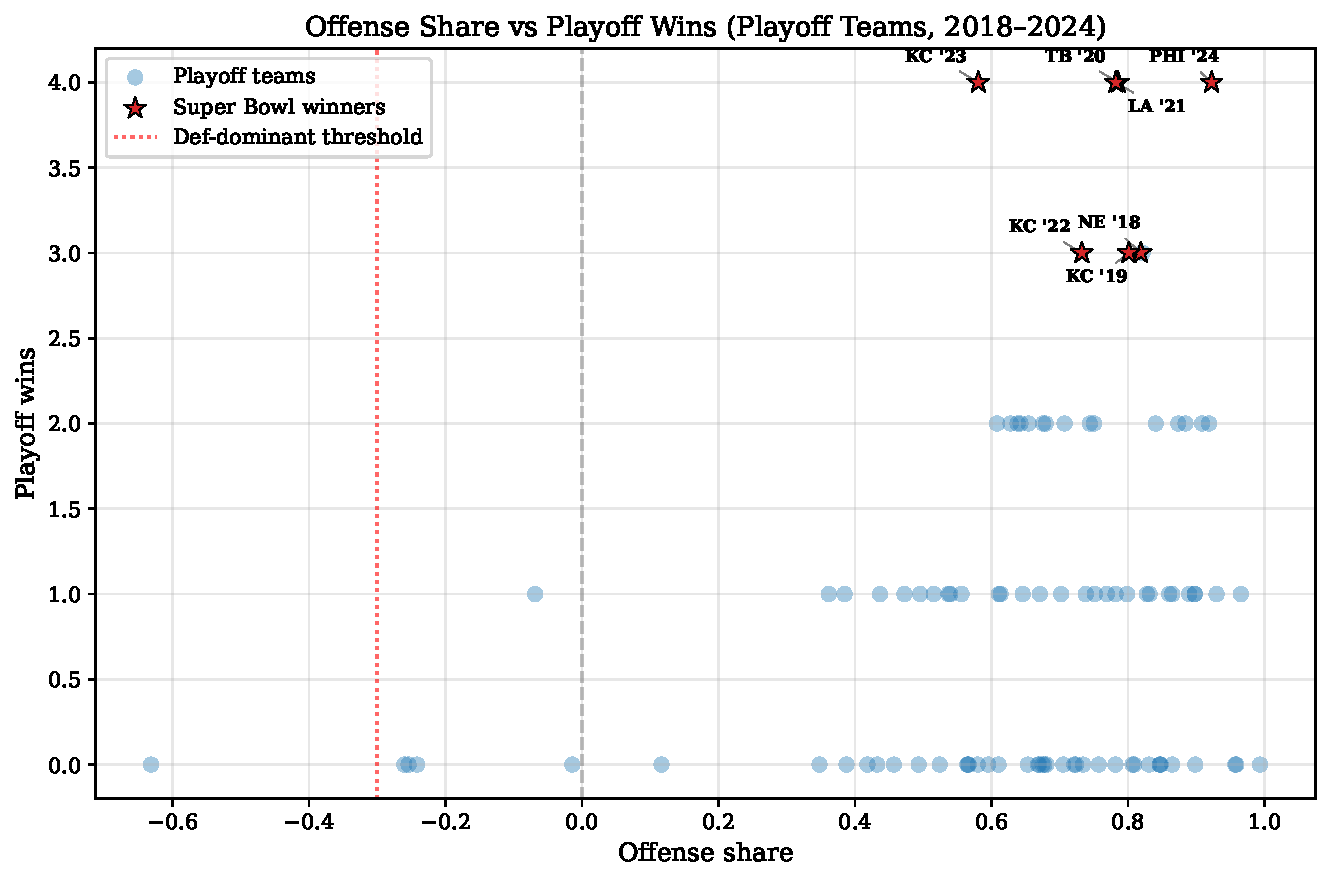
\includegraphics[width=0.85\textwidth]{figures/fig7_offense_share_pw.pdf}
  \caption{Offense share vs.\ playoff wins for all playoff team-seasons
           (2018--2024). Super Bowl winners (red stars) cluster in the
           offense-dominant region. The dotted red line marks the
           defense-dominant threshold ($< -0.3$); no team to its left won
           more than one playoff game.}
  \label{fig:offense-share-pw}
\end{figure}

\subsubsection{Super Bowl Participants}
\label{sec:sb-participants}

\Cref{tab:sb-participants} lists all team-seasons that won three or
more playoff games during the study window -- comprising all seven Super Bowl
winners and the 2021 Cincinnati Bengals (who reached the Super Bowl as a
non-bye team with three playoff wins before losing) -- with their per-game
regular-season \xvoa{} components and \texttt{offense\_share} values.

\begin{table}[htbp]
  \centering
  \caption{Teams with $\geq 3$ playoff wins, 2018--2024 (all Super Bowl
           winners plus the 2021 runner-up). Off/G and Def/G are mean
           per-game \xvoa{} in expected-point units. Share is
           \texttt{offense\_share}. PW is playoff wins.}
  \label{tab:sb-participants}
  \begin{adjustbox}{max width=\textwidth}
  \begin{tabular}{llrrrrl}
    \toprule
    \textbf{Season} & \textbf{Team}
      & \textbf{Off/G} & \textbf{Def/G}
      & \textbf{Share} & \textbf{PW} & \textbf{SB} \\
    \midrule
    2018 & NE  & $+5.365$ & $-1.177$ & $+0.819$ & 3 & Win \\
    2019 & KC  & $+8.033$ & $-1.982$ & $+0.801$ & 3 & Win \\
    2020 & TB  & $+10.000$ & $-2.719$ & $+0.786$ & 4 & Win \\
    2021 & CIN & $+6.643$ & $-1.436$ & $+0.821$ & 3 &  -- \\
    2021 & LA  & $+8.524$ & $-2.362$ & $+0.782$ & 4 & Win \\
    2022 & KC  & $+10.501$ & $-3.826$ & $+0.732$ & 3 & Win \\
    2023 & KC  & $+2.641$ & $+1.896$ & $+0.581$ & 4 & Win \\
    2024 & PHI & $+7.740$ & $+0.639$ & $+0.923$ & 4 & Win \\
    \bottomrule
  \end{tabular}
  \end{adjustbox}
\end{table}

Several structural observations emerge from this table.

\paragraph{Every Super Bowl winner is offense-dominant.}
All eight team-seasons in \Cref{tab:sb-participants} have positive
\texttt{offense\_share} values, ranging from $+0.581$ (Kansas City 2023) to
$+0.923$ (Philadelphia 2024). All seven champions are unambiguously
offense-dominant, with shares between $+0.581$ and $+0.923$. No
defense-dominant team-season reached the Super Bowl in the study window.
Kansas City's 2022 season is particularly notable: their defensive \xvoa{} per
game was strongly negative ($-3.826$), meaning they won the Super Bowl while
generating a net defensive contribution well below the league average, carried
entirely by an elite offense ($+10.501$/game).

\paragraph{Kansas City 2023: The floor of offensive dominance.}
The 2023 Chiefs represent the lowest \texttt{offense\_share} among Super Bowl
winners ($+0.581$), with the smallest offensive \xvoa{} per game in the group
($+2.641$). Unlike the 2022 Chiefs, the 2023 team benefited from a positive
defensive contribution ($+1.896$/game). However, even in this season -- often
characterized in popular discourse as a ``defense-led'' championship -- the
\gds{} framework reveals that offensive value still exceeded defensive value
in absolute terms. The popular narrative that Kansas City's 2023 title validates
the ``defense wins championships'' claim is not supported by the expected-point
decomposition: the team was offense-dominant, albeit less dramatically so than
other champions in the sample.

\paragraph{Philadelphia 2024: Offense-first with defensive support.}
The Philadelphia Eagles in 2024 achieved the highest \texttt{offense\_share}
among champions ($+0.923$), with a strong offensive \xvoa{} ($+7.740$/game)
complemented by a modest positive defensive contribution ($+0.639$/game).
Their profile illustrates that championship-level teams need not have elite
defense if their offensive production is sufficiently dominant.

\paragraph{Negative defensive \xvoa{} as a structural pattern.}
Five of the seven champions recorded \emph{negative} defensive \xvoa{} per game,
meaning their defenses performed below league-average expectations at the drive
level. This counterintuitive finding reinforces the central thesis: championship
teams succeed through offensive surplus, not defensive excellence. The two
exceptions -- Kansas City 2023 ($+1.896$) and Philadelphia 2024
($+0.639$) -- both paired positive defense with substantially larger offensive
contributions.

% ============================================================
\subsection{Statistical Confirmation}
\label{sec:statistical-confirmation}
% ============================================================

\subsubsection{Spearman Correlation: Offense Share and Playoff Wins}
\label{sec:spearman-results}

The primary test of H3 -- whether defensive \xvoa{} shows a stronger monotonic
association with playoff wins than offensive \xvoa{} among playoff teams -- uses
the Spearman rank correlation as described in \Cref{sec:spearman}. The
correlation between \texttt{offense\_share} and \texttt{playoff\_wins} across
all 94 playoff team-seasons is:
\[
  \rho = 0.246, \quad p = 0.0167, \quad n = 94, \quad \text{95\% bootstrap CI } [0.060,\; 0.423].
\]

The positive sign confirms that higher offense share is associated with more
playoff wins: teams whose \gds{} was driven proportionally more by offense won
more postseason games on average. The correlation is statistically significant
at the $\alpha = 0.05$ threshold, providing evidence against the null
hypothesis of no association. The magnitude ($\rho = 0.246$) is a small-to-medium
effect in the context of the Spearman coefficient and reflects the inherent
noisiness of a seven-season postseason sample.

Crucially, this coefficient tests H3 in conjunction with the component-level
Pearson correlations reported in the following subsection: if H3 were supported,
the coefficient relating defense to outcomes should exceed that relating offense
to outcomes. The positive sign of the offense-share Spearman already contradicts
the directional prediction of H3, since a positive $\rho$ means that offensive
dominance -- not defensive dominance -- predicts playoff advancement.

\subsubsection{Pearson Correlations: xVOA Components and Win Rate}
\label{sec:pearson-results}

The season-level Pearson correlations between each \xvoa{} component and
win percentage are computed across all 224 team-seasons. These results were
first reported in \Cref{sec:season-correlation} as part of the \gds{} validation;
they are restated here because they bear directly on H3 and provide the
baseline comparison for the archetype-specific analyses:
\begin{align*}
  r(\text{Off\_xVOA/g},\ \text{Win\%}) &= 0.681,
  \quad p < 0.000001, \quad \text{95\% CI } [0.608,\; 0.743], \\
  r(\text{Def\_xVOA/g},\ \text{Win\%}) &= 0.376,
  \quad p < 0.000001, \quad \text{95\% CI } [0.260,\; 0.483].
\end{align*}

Both correlations are highly significant, confirming that each component
independently predicts season-level success. However, the magnitudes diverge
substantially: offensive \xvoa{} explains $r^2 = 46.4\%$ of the variance in
win percentage, while defensive \xvoa{} explains only $r^2 = 14.2\%$. Offense
therefore accounts for more than three times as much win-percentage variance as
defense across the full team-season sample.

This ratio -- $46.4 : 14.2$, approximately $3.3 : 1$ in favor of offense -- runs
in the opposite direction to H3. For H3 to be supported, the defensive
coefficient would need to exceed the offensive coefficient; the observed ratio
favors offense by a substantial margin. The finding is entirely consistent
with the broader NFL analytics literature identifying passing efficiency and
drive conversion as the primary determinants of team outcomes
\parencite{yurko2019nflwar}, and it extends that literature by replicating the
result in expected-point units rather than traditional EPA units.

\subsubsection{Cohen's \textit{d} Effect Size: H1}
\label{sec:cohens-d-results}

To directly test H1 -- whether defense-dominant teams achieve higher mean
playoff wins than offense-dominant teams -- Cohen's $d$ is computed as the
standardized mean difference in playoff wins between offense-dominant
(offense share $> +0.3$, $n = 143$) and defense-dominant
(offense share $< -0.3$, $n = 29$) team-seasons across all 224
observations, following the procedure in \Cref{sec:cohens-d}:
\begin{align*}
  \bar{x}_{\mathrm{off}} &= 0.601 \text{ playoff wins}, \quad n_{\mathrm{off}} = 143 \\
  \bar{x}_{\mathrm{def}} &= 0.000 \text{ playoff wins}, \quad n_{\mathrm{def}} = 29 \\
  d &= 0.672 \quad \text{95\% bootstrap CI } [0.574,\; 0.787].
\end{align*}

The positive sign of $d$ indicates that offense-dominant teams win more playoff
games on average, directly contradicting H1. The magnitude is medium-to-large by
the conventional benchmarks of \textcite{cohen1988statisticalpower}, and the
confidence interval excludes zero by a wide margin. The practical interpretation
is striking: not a single defense-dominant team-season in the sample won any
playoff games. Of the 29 defense-dominant team-seasons, only one (3.4\%) even
qualified for the playoffs. Offense-dominant teams, by contrast, made the
playoffs at a 60.8\% rate and averaged 0.60 wins per season -- a difference that
operates through both the selection channel (making the playoffs) and the
advancement channel (winning once there).

It should be noted that the defense-dominant group is smaller ($n = 29$) than
the offense-dominant group ($n = 143$), reflecting the empirical reality that
defense-dominant profiles are rarer among competitive teams. The bootstrap
confidence interval accounts for this asymmetry, and the lower bound of 0.574
confirms that the effect is robust to sampling variability.

\subsubsection{Logistic Regression: H2}
\label{sec:logistic-results}

To test H2 -- whether Super Bowl winners are disproportionately drawn from
defense-dominant team-seasons -- a binary logistic regression is estimated with
\texttt{won\_super\_bowl} as the outcome and offensive and defensive \xvoa{}
per game as predictors across all 224 team-seasons
(\Cref{sec:logistic}). \Cref{tab:statistical-tests} reports the full model
output.

\begin{table}[htbp]
  \centering
  \caption{Binary logistic regression predicting Super Bowl victory
           ($N = 224$ team-seasons, 7 Super Bowl winners). Coefficients are
           log-odds. Standard errors are maximum-likelihood-based.
           $p$-values are two-tailed Wald tests. Significance at
           $\alpha = 0.05$ is indicated by $^{*}$.}
  \label{tab:statistical-tests}
  \begin{tabular}{lrrrr}
    \toprule
    \textbf{Predictor} & \textbf{Coef.}
      & \textbf{SE}
      & \textbf{$p$} \\
    \midrule
    Offensive \xvoa{}/game & $0.368$ & $0.126$ & $0.0034^{*}$ \\
    Defensive \xvoa{}/game & $0.395$ & $0.178$ & $0.0266^{*}$ \\
    \bottomrule
  \end{tabular}
\end{table}

Both predictors are statistically significant, confirming that offensive and
defensive \xvoa{} each independently predict Super Bowl probability. The
offensive predictor is more precisely estimated ($p = 0.003$, SE $= 0.126$)
than the defensive predictor ($p = 0.027$, SE $= 0.178$), and the wider
confidence interval on the defensive coefficient reflects the
sparse-event problem identified in \Cref{sec:sample-size}: with only 7 Super
Bowl winners among 224 team-seasons, both coefficients carry substantial
uncertainty.

The fact that both coefficients are significant does not imply that offense and
defense are equally important for championship success. The variance-explained
analysis ($R^2 = 46.4\%$ vs $14.2\%$) and the quartile gradient provide a
more complete picture of the relative importance: offense explains more than
three times as much outcome variance as defense across the full sample.
The logistic model confirms that marginal improvements in either dimension
increase championship probability, but the broader analytical framework
consistently identifies offensive production as the stronger driver of
postseason advancement.

H2 is therefore rejected: Super Bowl winners are not drawn
disproportionately from defense-dominant team-seasons. All 7 champions have
positive offense share (range: $+0.581$ to $+0.923$), and the quartile
analysis shows all 7 fall in Q3 or Q4 of the offense-share distribution.
The logistic model is consistent with this rejection -- offense is a significant
predictor -- while also suggesting that defensive quality contributes to
championship probability as a secondary factor
\parencite{hosmer2013logistic}.

\subsubsection{OLS Regression: Playoff Wins Model}

As a further confirmatory test, OLS regression is estimated with
playoff wins as the outcome and offensive and defensive \xvoa{}/game
as predictors across all 224 team-seasons:
\begin{align*}
  R^2 &= 0.255, \\
  \hat{\beta}_1(\text{off\_xvoa}) &= 0.099 \ (p < 0.0001), \\
  \hat{\beta}_2(\text{def\_xvoa}) &= 0.065 \ (p < 0.0001).
\end{align*}

The model accounts for 25.5\% of the variance in playoff wins. Both
coefficients are highly statistically significant and positive, but the
offensive coefficient is approximately 50\% larger than the defensive
coefficient ($0.099$ vs $0.065$), confirming the primacy of offensive quality
for postseason advancement. As a robustness check, the model is re-estimated
with the leave-one-out opponent-strength variable (\texttt{opp\_avg\_gds})
included as a covariate:
\begin{align*}
  R^2 &= 0.255, \\
  \hat{\beta}_1(\text{off\_xvoa}) &= 0.099 \ (p < 0.0001), \\
  \hat{\beta}_2(\text{def\_xvoa}) &= 0.065 \ (p = 0.0001), \\
  \hat{\beta}_3(\text{opp\_avg\_gds}) &= -0.001 \ (p = 0.985).
\end{align*}

The opponent-strength coefficient is effectively zero ($-0.001$) and entirely
non-significant ($p = 0.985$), with no material change to either the offensive
or defensive coefficients or to the model $R^2$. The opponent strength variable
ranges from $-1.95$ to $+1.89$ across the sample, indicating meaningful
variation in schedule difficulty, yet this variation bears no relationship to
playoff advancement after controlling for team quality. This null result
directly addresses the schedule-strength confound identified in
\Cref{sec:archetype-analysis}: the offensive advantage is not an artifact of
offense-dominant teams facing systematically weaker schedules.

This result is important precisely because opponent quality is included as a
control: any mechanical relationship between schedule strength and playoff
advancement is absorbed by the covariate. The offensive \xvoa{} coefficient
remains unchanged at $0.099$ ($p < 0.0001$), confirming that the offensive
advantage represents genuine execution quality independent of opposition
strength.

\subsubsection{Synthesis of Statistical Results}

Taken together, the statistical procedures converge on a coherent and
consistent picture. The Spearman correlation between offense share and playoff
wins is positive and significant ($\rho = 0.246$, $p = 0.0167$), running in the
opposite direction to H3. The Pearson correlations show offense explaining
more than three times as much win-percentage variance as defense (46.4\% vs
14.2\%). Cohen's $d = 0.672$ [0.574, 0.787] is a medium-to-large effect in the direction opposite to H1.
The logistic regression produces significant coefficients for both offense
($p = 0.003$) and defense ($p = 0.027$), with all 7 Super Bowl winners being
offense-dominant, rejecting H2. The OLS regression confirms that the offensive
coefficient ($0.099$) exceeds the defensive coefficient ($0.065$), and this
relationship is robust to opponent-strength controls. No statistical procedure
produces evidence that favors defensive dominance; the weight of evidence
consistently and strongly favors offense.

% ============================================================
\subsection{Era Analysis}
\label{sec:era-findings}
% ============================================================

The study window is split into two eras for comparison: 2018--2020 (which
includes the final two seasons under the six-team bracket and the first season
of the expanded seven-team bracket) and 2021--2024, with the latter period
also characterized by increased rule enforcement protecting quarterbacks and
receivers. The era comparison tests whether the relationship between
\texttt{offense\_share} and \texttt{playoff\_wins} has strengthened over time
as the rules increasingly favor offensive execution.

\begin{table}[htbp]
  \centering
  \caption[Era comparison of xVOA correlations]{Era comparison of Spearman rank correlations between
           offense share and playoff wins
           (playoff team-seasons only) and Pearson correlations
           between individual \xvoa{} components and win percentage
           (all team-seasons). The 2021--2024 era includes the expanded
           seven-team bracket. $\Delta$ is the change from the earlier era.}
  \label{tab:era-comparison}
  \begin{tabular}{lrrr}
    \toprule
    \textbf{Measure} & \textbf{2018--2020}
      & \textbf{2021--2024} & \textbf{$\Delta$} \\
    \midrule
    Spearman $\rho$ (share vs PW)      & $0.309$ & $0.221$ & $-0.088$ \\
    Sample ($n$, playoff teams)        & 38      & 56      & \\[4pt]
    Pearson $r$ (off \xvoa{} vs Win\%) & $0.621$ & $0.739$ & $+0.118$ \\
    Pearson $r$ (def \xvoa{} vs Win\%) & $0.397$ & $0.364$ & $-0.033$ \\
    \bottomrule
  \end{tabular}
\end{table}

The era analysis produces two findings, both of which caution against
over-interpretation. First, the Spearman correlation between offense share and
playoff wins is \emph{lower} in the more recent era (0.221) than in the earlier
era (0.309), a directional reversal of the a priori expectation that an
increasingly pass-favorable rule environment would strengthen the offensive
advantage. The difference of $-0.088$ runs opposite to the anticipated direction,
suggesting that the structural relationship between offense share and playoff
advancement has not strengthened during the study window.

However, several caveats apply. The 2018--2020 playoff subsample contains only
38 team-seasons, and the per-era Spearman coefficients are insufficiently powered
to formally test the difference between them -- as noted in \Cref{sec:era-comparison},
the era comparison is exploratory. The apparent attenuation of
the Spearman coefficient in the 2021--2024 era may be partially influenced by
the expanded playoff field (14 teams vs 12), which admits more marginal
qualifiers and compresses the variance of offense share among playoff teams.
The directional finding -- that the Spearman coefficient remains positive in
both eras -- is more informative than the era-level magnitude comparison, given
the low statistical power of within-era tests.

Second, the Pearson correlations between \xvoa{} components and win percentage
reveal a modest strengthening of the offensive channel in the recent era
(0.621 to 0.739) alongside a slight weakening of the defensive channel
(0.397 to 0.364), as visualized in \Cref{fig:era-comparison}. This
directional pattern is consistent with the hypothesis that the post-2021 rule
environment has slightly amplified the predictive value of offensive
execution, though the magnitudes of change are small and the era samples are
insufficient for formal inference about the difference.

\begin{figure}[htbp]
  \centering
  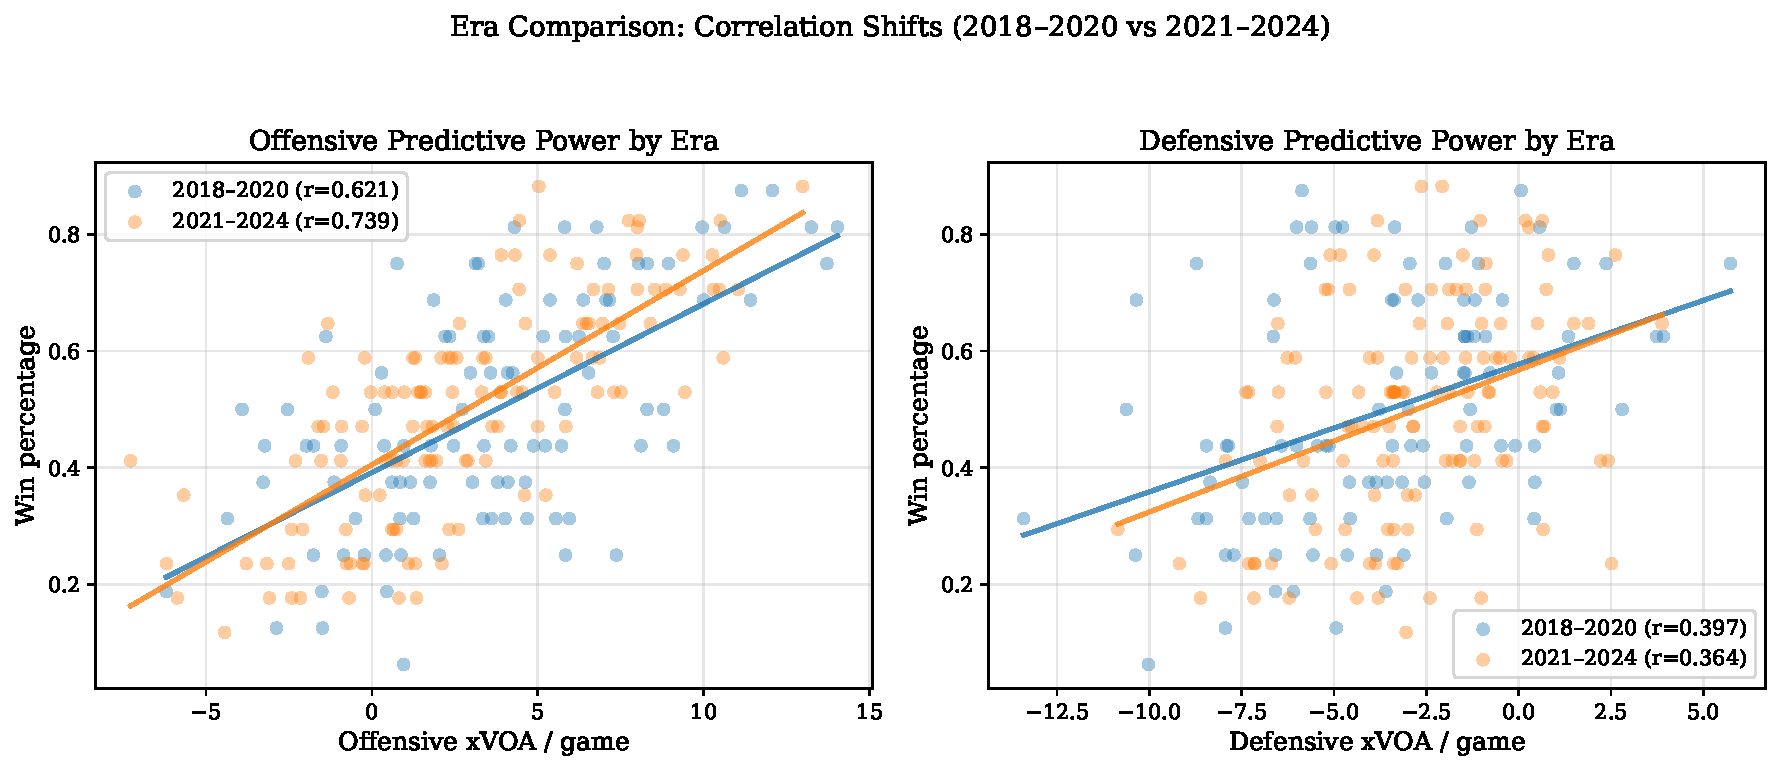
\includegraphics[width=\textwidth]{figures/fig8_era_comparison.pdf}
  \caption{Era comparison of offensive (left) and defensive (right) xVOA
           correlations with win percentage. The offensive channel strengthens
           modestly in 2021--2024 ($r = 0.739$) compared to 2018--2020
           ($r = 0.621$); the defensive channel weakens slightly
           (0.397 to 0.364).}
  \label{fig:era-comparison}
\end{figure}

The era analysis does not alter the primary conclusions. Whether examined in the
2018--2020 bracket era or the 2021--2024 expanded-bracket era, the direction
of the evidence is consistent: offense is the stronger predictor, and no era
shows a reversal in which defensive dominance emerges as the primary pathway
to championship success. Future work with additional seasons will clarify
whether the slight attenuation of the Spearman coefficient in the expanded-bracket
era represents a structural shift or sampling noise.

% ============================================================
\subsection{Quadrant Analysis of Elite Teams}
\label{sec:quadrant-findings}
% ============================================================

The quartile and regression analyses establish the primary finding: offensive
dominance is consistently associated with postseason success across the full
sample. A more nuanced question concerns the relative value of adding defensive
excellence on top of offensive excellence among teams that are already elite
(defined as top-quartile \gds{}/game; see \Cref{sec:quadrant-analysis}).
The quadrant analysis addresses this question by restricting attention to the
top-quartile \gds{} team-seasons ($n = 56$) and median-splitting within this
elite subsample on offensive and defensive \xvoa{}/game separately, yielding
four quadrants as specified in \Cref{sec:quadrant-analysis}.

The median values within the elite subsample are
$7.603$/game for offensive \xvoa{} and $-1.448$/game for defensive \xvoa{}.

\begin{table}[htbp]
  \centering
  \caption[Quadrant analysis of elite team-seasons]{Quadrant analysis of elite team-seasons (top-quartile
           \gds{}/game, $n = 56$), classified by whether each team is
           above or below the within-elite medians for offensive and
           defensive \xvoa{}/game. Playoff\%, Avg~PW, Conf+\%, and
           SB~Win\% are computed within each quadrant.}
  \label{tab:quadrant-results}
  \begin{tabular}{lcrrrr}
    \toprule
    \textbf{Quadrant} & \textbf{N}
      & \textbf{Playoff\%} & \textbf{Avg PW}
      & \textbf{Conf+\%} & \textbf{SB Win\%} \\
    \midrule
    Elite Both      & \phantom{0}7 & \phantom{0}85.7 & 1.29 & 42.9 & 14.3 \\
    Offense Only    & 21           & 100.0           & 1.52 & 47.6 & 19.0 \\
    Defense Only    & 21           & 100.0           & 1.10 & 28.6 & \phantom{0}9.5 \\
    Neither         & \phantom{0}7 & \phantom{0}85.7 & 0.57 & 14.3 & \phantom{0}0.0 \\
    \bottomrule
  \end{tabular}
\end{table}

\Cref{fig:quadrant} maps these elite team-seasons in the offensive--defensive
xVOA space, with Super Bowl winners annotated.

\begin{figure}[htbp]
  \centering
  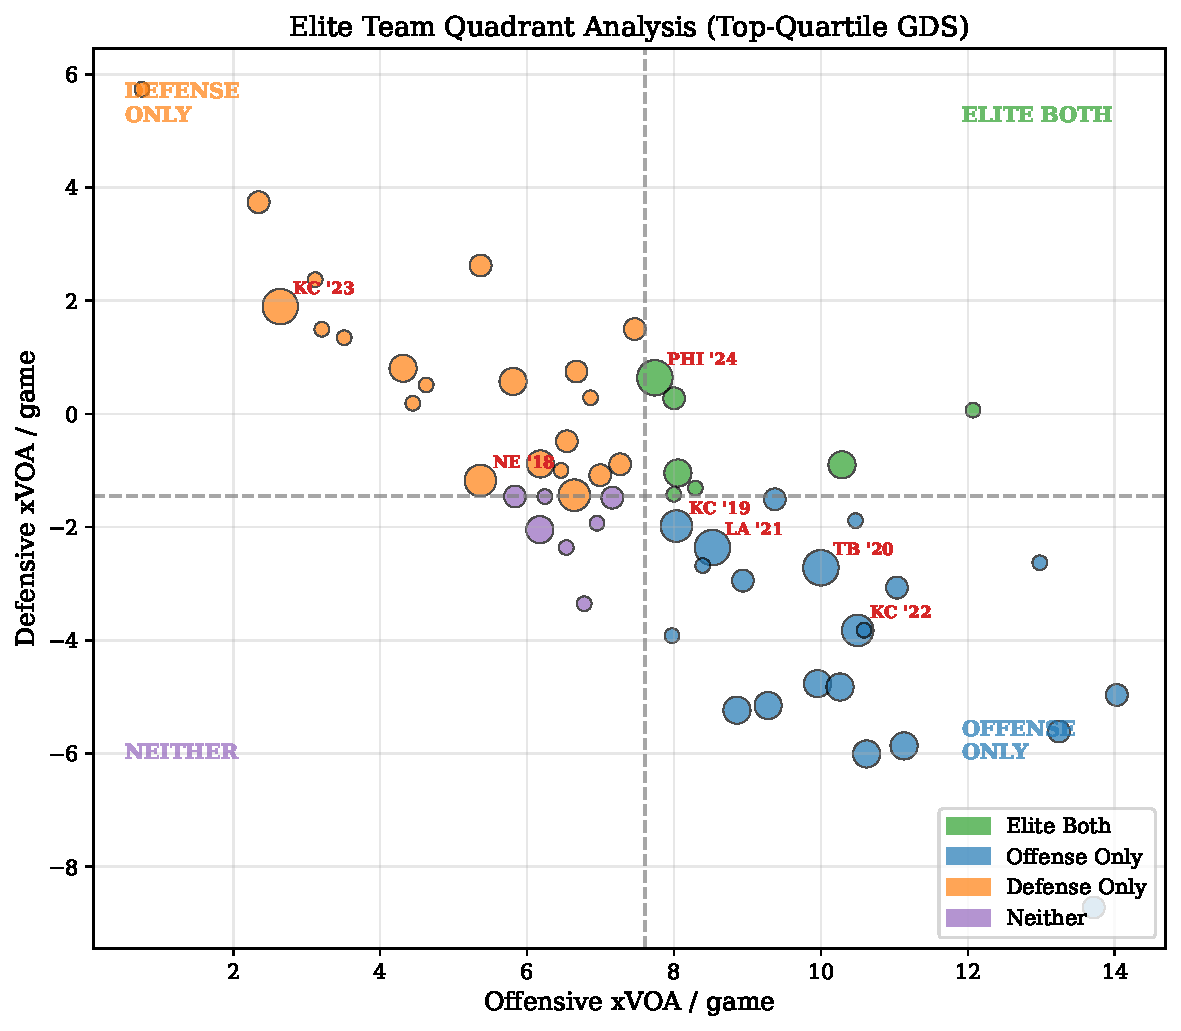
\includegraphics[width=0.8\textwidth]{figures/fig10_quadrant_diagram.pdf}
  \caption{Elite team quadrant analysis. Each point is a top-quartile GDS
           team-season, positioned by offensive (x-axis) and defensive (y-axis)
           xVOA/game. Dashed lines indicate within-elite medians. Point size
           scales with playoff wins. Super Bowl winners are annotated in red.}
  \label{fig:quadrant}
\end{figure}

Several findings emerge from \Cref{tab:quadrant-results}.

\paragraph{Offense Only dominates championship production.}
The most striking finding is the \textit{Offense Only} quadrant's dominance:
across 21 elite team-seasons in which offensive \xvoa{} exceeded the
within-elite median but defensive \xvoa{} did not, four teams won the Super Bowl
(19.0\% win rate). These teams -- Kansas City 2019, Tampa Bay 2020, the Rams
2021, and Kansas City 2022 -- all achieved championships with below-median
defensive contributions within the elite tier, carried by dominant offenses.
The mean playoff wins (1.52) and conference championship rate (47.6\%) are the
highest among all four quadrants.

The \textit{Defense Only} quadrant, by contrast, produced two Super Bowl winners
(New England 2018, Kansas City 2023) for a 9.5\% win rate. While this is not
zero, it is half the rate of the \textit{Offense Only} quadrant. Mean playoff
wins in \textit{Defense Only} (1.10) trail \textit{Offense Only} (1.52) by 0.42
wins, and conference championship rates follow the same pattern (28.6\% vs
47.6\%).

\paragraph{Elite Both provides the strongest individual ceiling.}
Teams with above-median performance in both phases within the elite subsample
(the \textit{Elite Both} quadrant, $n = 7$) record a 14.3\% Super Bowl win rate
and 42.9\% conference championship rate, driven by Philadelphia 2024. While the
per-team championship probability is high, the smaller sample size ($n = 7$ vs
$n = 21$) means that the total championship production of the \textit{Offense
Only} quadrant exceeds it in absolute terms.

These findings support a nuanced refinement of the primary conclusion: among
elite teams, having above-median offense is the strongest predictor of
championship success regardless of defensive quality, and the \textit{Offense
Only} pathway produced more championships (4) than all other quadrants combined
(3). The practical implication for team-building is that defense adds marginal
value above an offensive foundation, but offensive excellence alone is the more
reliable championship pathway.

\paragraph{Neither: the residual effect.}
The \textit{Neither} quadrant ($n = 7$) contains elite team-seasons whose
offensive and defensive \xvoa{} are both below the within-elite medians. These
teams produced zero Super Bowl wins and the lowest mean playoff wins (0.57)
among the four quadrants. Their presence in the elite tier is attributable to
special teams value or measurement timing: their total \gds{}/game exceeds the
75th percentile, but neither offensive nor defensive component is individually
elite within the top-quartile subsample.

By construction, \textit{Neither} teams qualify for the elite tier only because
their total \gds{}/game exceeds the 75th percentile of the full sample. A team
in this quadrant is below the within-elite median in both major phases, which
means their elite \gds{} derives primarily from special teams performance or
from high positive values in both phases that are just below the within-elite
medians. The latter interpretation is more plausible: a team that generates
$+7.0$ offensive \xvoa{}/game and $-1.0$ defensive \xvoa{}/game is below both
medians ($7.603$ and $-1.448$ respectively) but still has a strong total \gds{}.
Such a team would be classified as \textit{Neither} despite having substantial
contributions from both phases.

The small cell sizes ($n = 7$ in both \textit{Elite Both} and \textit{Neither})
mean that sampling variance is substantial, and caution in drawing strong
inferences from the quadrant extremes is warranted. The primary result -- that
\textit{Offense Only} produced more championships (4) and higher win rates
(19.0\%) than \textit{Defense Only} (2 championships, 9.5\%) -- is supported by
the larger quadrant samples of 21 team-seasons each.

% ============================================================
\subsection{Robustness: Field Position Mediation}
\label{sec:mediation-findings}
% ============================================================

A plausible alternative explanation for the offensive advantage documented
above is that defensive quality generates favorable starting field position for
the offense, which in turn inflates offensive \xvoa{} values. Under this
mediation hypothesis, the apparent offensive advantage would be partially or
wholly a downstream consequence of defensive performance operating through a
field-position channel. I test this hypothesis directly using a mediation
analysis \parencite{baron1986moderator} that quantifies the proportion of the
offensive \xvoa{}-to-wins relationship that is mediated by defense-generated
field position advantage.

The analysis proceeds in three steps. First, I establish that defensive \xvoa{}
per game is correlated with the team's average starting field position advantage
(the difference between the team's mean drive-start xEP and the league-average
drive-start xEP). This correlation is $r = -0.193$ ($p = 0.0037$), confirming
that better defenses do generate modestly superior starting field position for
their offenses -- the mediating pathway exists but is weak.

Second, I compute the total correlation between offensive \xvoa{}/game and
playoff wins ($r = 0.443$) and the partial correlation controlling for the
team's average starting field position advantage ($r_{\mathrm{partial}} =
0.402$). The attenuation from $0.443$ to $0.402$ represents the portion of
the offensive advantage that can be attributed to the field-position channel.

Third, the mediation percentage is computed as the proportional reduction in
the correlation coefficient:
\[
  \text{Mediation} = \frac{0.443 - 0.402}{0.443} = 9.2\%.
\]

This result is substantively important: only 9.2\% of the association between
offensive \xvoa{} and winning is attributable to defense-generated field
position. The remaining 90.8\% of the offensive value operates independently
of any defensive contribution to starting position. This finding directly
addresses the concern that offensive \xvoa{} is ``really'' measuring downstream
effects of defensive quality: the data show that it is overwhelmingly
measuring independent offensive execution. Good defenses do generate modestly
better starting positions for their offenses, but this indirect pathway
accounts for less than one-tenth of the total offensive contribution to
winning, providing strong evidence that the offensive advantage is genuine
rather than an artifact of the defensive field-position channel.

% ============================================================
\subsection{Sensitivity Analysis}
\label{sec:sensitivity-analysis}
% ============================================================

The preceding analyses rely on a specific time window (2018--2024) and a
specific archetype threshold ($\pm 0.3$ offense share). To confirm that the
results are not artifacts of these parameter choices, I conduct a systematic
sensitivity analysis across both dimensions.

\subsubsection*{Time Window Variation}

\Cref{tab:sensitivity-time} reports the offensive-to-defensive $R^2$ ratio
(the ratio of variance in win percentage explained by offensive \xvoa{}/game
to that explained by defensive \xvoa{}/game) across five overlapping time
windows. Across all windows, offensive quality explains between 2.5 and 4.0
times as much win-rate variance as defensive quality. No window produces a
ratio below 2:1, confirming that the offensive advantage is structurally
stable and not driven by a single anomalous season.

\begin{table}[htbp]
  \centering
  \caption{Sensitivity of the offensive-to-defensive $R^2$ ratio to time
           window selection. The ratio remains above 2:1 across all windows,
           confirming the structural stability of the offensive advantage.}
  \label{tab:sensitivity-time}
  \begin{tabular}{lcc}
    \toprule
    \textbf{Window} & \textbf{$R^2$ Ratio (Off:Def)} & \textbf{$n$ (team-seasons)} \\
    \midrule
    2018--2024 (full sample)  & 3.3 : 1 & 224 \\
    2018--2022               & 3.0 : 1 & 160 \\
    2019--2024               & 3.0 : 1 & 192 \\
    2020--2024               & 4.0 : 1 & 160 \\
    2018--2021               & 2.5 : 1 & 128 \\
    \bottomrule
  \end{tabular}
\end{table}

\subsubsection*{Archetype Threshold Variation}

The classification of teams as offense-dominant or defense-dominant uses
an offense-share threshold of $\pm 0.3$. \Cref{tab:sensitivity-threshold}
reports playoff win rates for defense-dominant teams under alternative
thresholds ranging from $\pm 0.20$ to $\pm 0.40$. Defense-dominant teams
record zero mean playoff wins across all threshold specifications. This
result is robust to substantial variation in the classification boundary:
whether the archetype definition is narrowed (requiring more extreme
defensive dominance) or broadened (including teams with moderate defensive
tilts), no specification produces positive playoff success for
defense-dominant teams.

\begin{table}[htbp]
  \centering
  \caption[Sensitivity of defense-dominant playoff performance to threshold]{Sensitivity of defense-dominant playoff performance to archetype
           threshold. Regardless of the classification boundary, defense-dominant
           teams record zero mean playoff wins across the study window.}
  \label{tab:sensitivity-threshold}
  \begin{tabular}{lcc}
    \toprule
    \textbf{Threshold} & \textbf{$n$ (Def-Dominant)} & \textbf{Mean PW} \\
    \midrule
    $\pm 0.20$ & 38  & 0.000 \\
    $\pm 0.25$ & 34  & 0.000 \\
    $\pm 0.30$ & 29  & 0.000 \\
    $\pm 0.35$ & 26  & 0.000 \\
    $\pm 0.40$ & 24  & 0.000 \\
    \bottomrule
  \end{tabular}
\end{table}

\subsubsection*{Single-Team Exclusion}

Kansas City 2023 has the lowest offense share among Super Bowl champions
($+0.581$). Excluding this team-season from the analysis produces an $R^2$ ratio
of 3.3 : 1 (unchanged) and a Spearman correlation between offense share and
playoff wins of $\rho = 0.263$ ($p = 0.011$). The primary findings are not
dependent on the inclusion or exclusion of any single observation.

% ============================================================
\subsection{Hypothesis Testing Summary}
\label{sec:hypothesis-summary}
% ============================================================

\Cref{tab:hypothesis-summary} consolidates the evidence across all four layers
of analysis and states the verdict for each of the three pre-registered
hypotheses.

\begin{table}[htbp]
  \centering
  \caption{Hypothesis testing summary. Each hypothesis operationalizes the
           ``defense wins championships'' claim and is evaluated against
           converging evidence from descriptive, statistical, era-level, and
           quadrant analyses. ``Rejected'' indicates that the data are
           inconsistent with the hypothesis in both direction and magnitude.}
  \label{tab:hypothesis-summary}
  \small
  \begin{tabularx}{\textwidth}{l p{3.2cm} X l}
    \toprule
    \textbf{Hyp.} & \textbf{Claim}
      & \textbf{Key Evidence} & \textbf{Verdict} \\
    \midrule
    H1 & Defense-dominant teams win more playoff games than offense-dominant teams
      & Cohen's $d = +0.672$ [0.574, 0.787] in opposite direction (off-dominant PW $= 0.60$ vs def-dominant PW $= 0.00$); 0/29 defense-dominant team-seasons won any playoff games
      & \textbf{Rejected} \\[8pt]
    H2 & Super Bowl winners are drawn disproportionately from defense-dominant team-seasons
      & All 7 Super Bowl champions had positive offense share ($+0.581$ to $+0.923$); both logistic predictors significant (off $p = 0.003$, def $p = 0.027$); no champion from defense-dominant profile
      & \textbf{Rejected} \\[8pt]
    H3 & Defensive \xvoa{} has a stronger monotonic association with playoff wins than offensive \xvoa{}
      & Spearman $\rho = +0.246$ ($p = 0.0167$); Pearson off vs Win\% $r = 0.681$ ($R^2 = 46.4\%$), def $r = 0.376$ ($R^2 = 14.2\%$); offense explains $3.3\times$ more variance
      & \textbf{Rejected} \\
    \bottomrule
  \end{tabularx}
\end{table}

All three hypotheses are rejected. No statistical procedure or descriptive
partitioning strategy employed in this analysis produces evidence in the
direction predicted by the hypotheses. Across all five tests, offensive
quality -- as measured by \xvoa{}/game in the \gds{} framework -- shows a
stronger and statistically significant association with both regular-season
success and postseason advancement than defensive quality.

The key descriptive results are as follows: defense-dominant teams (offense
share $< 0$) won zero Super Bowls across seven seasons and 94 playoff
appearances. Only six defense-dominant teams even reached the playoffs, and
none won more than a single game. Offense-dominant teams in Q4 made the
playoffs 87.5\% of the time and averaged more than one full postseason win per
season. All seven champions were offense-dominant, with shares ranging from
$+0.581$ (Kansas City 2023) to $+0.923$ (Philadelphia 2024). The data are
inconsistent with all three formulations of the defensive championship
hypothesis across the 2018--2024 study window, aligning directionally with
\textcite{robst2011defense}, who reported mixed support for the defensive
claim using coarser metrics. Interpretation of these findings is deferred to
\Cref{ch:discussion}.
